\section{Livros}

\begin{frame}[fragile]{The Art of Computer Programming}

    \begin{minipage}{0.45\textwidth}
        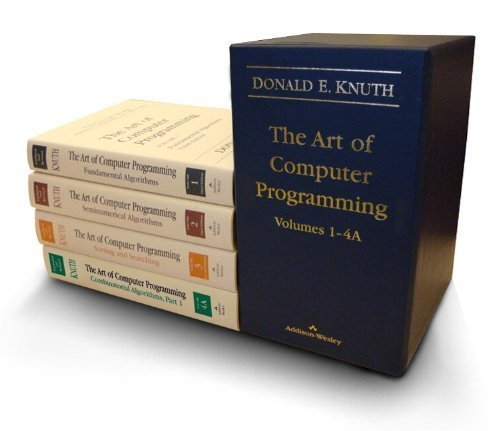
\includegraphics[scale=0.25]{knuth.jpg}
    \end{minipage}
    \begin{minipage}{0.45\textwidth}
        \begin{small}
            \begin{tabularx}{0.95\textwidth}{lX}
                \textbf{Autor:} & Donald E. Knuth \\
                \textbf{1ª Edição:} & 1968 \\
                \textbf{Volumes:} & 4 \\
                \textbf{Páginas:} & 3168 \\
                \textbf{Nível:} & Avançado \\
            \end{tabularx}
        \end{small}
    \end{minipage}

    Série clássica de livros sobre algoritmos, ainda inacabada. Apresenta os algoritmos de
    forma detalhada e analítica, com diversas referências à trabalhos científicos.

\end{frame}

\begin{frame}[fragile]{Algoritmos: Teoria e Prática}

    \begin{minipage}{0.4\textwidth}
        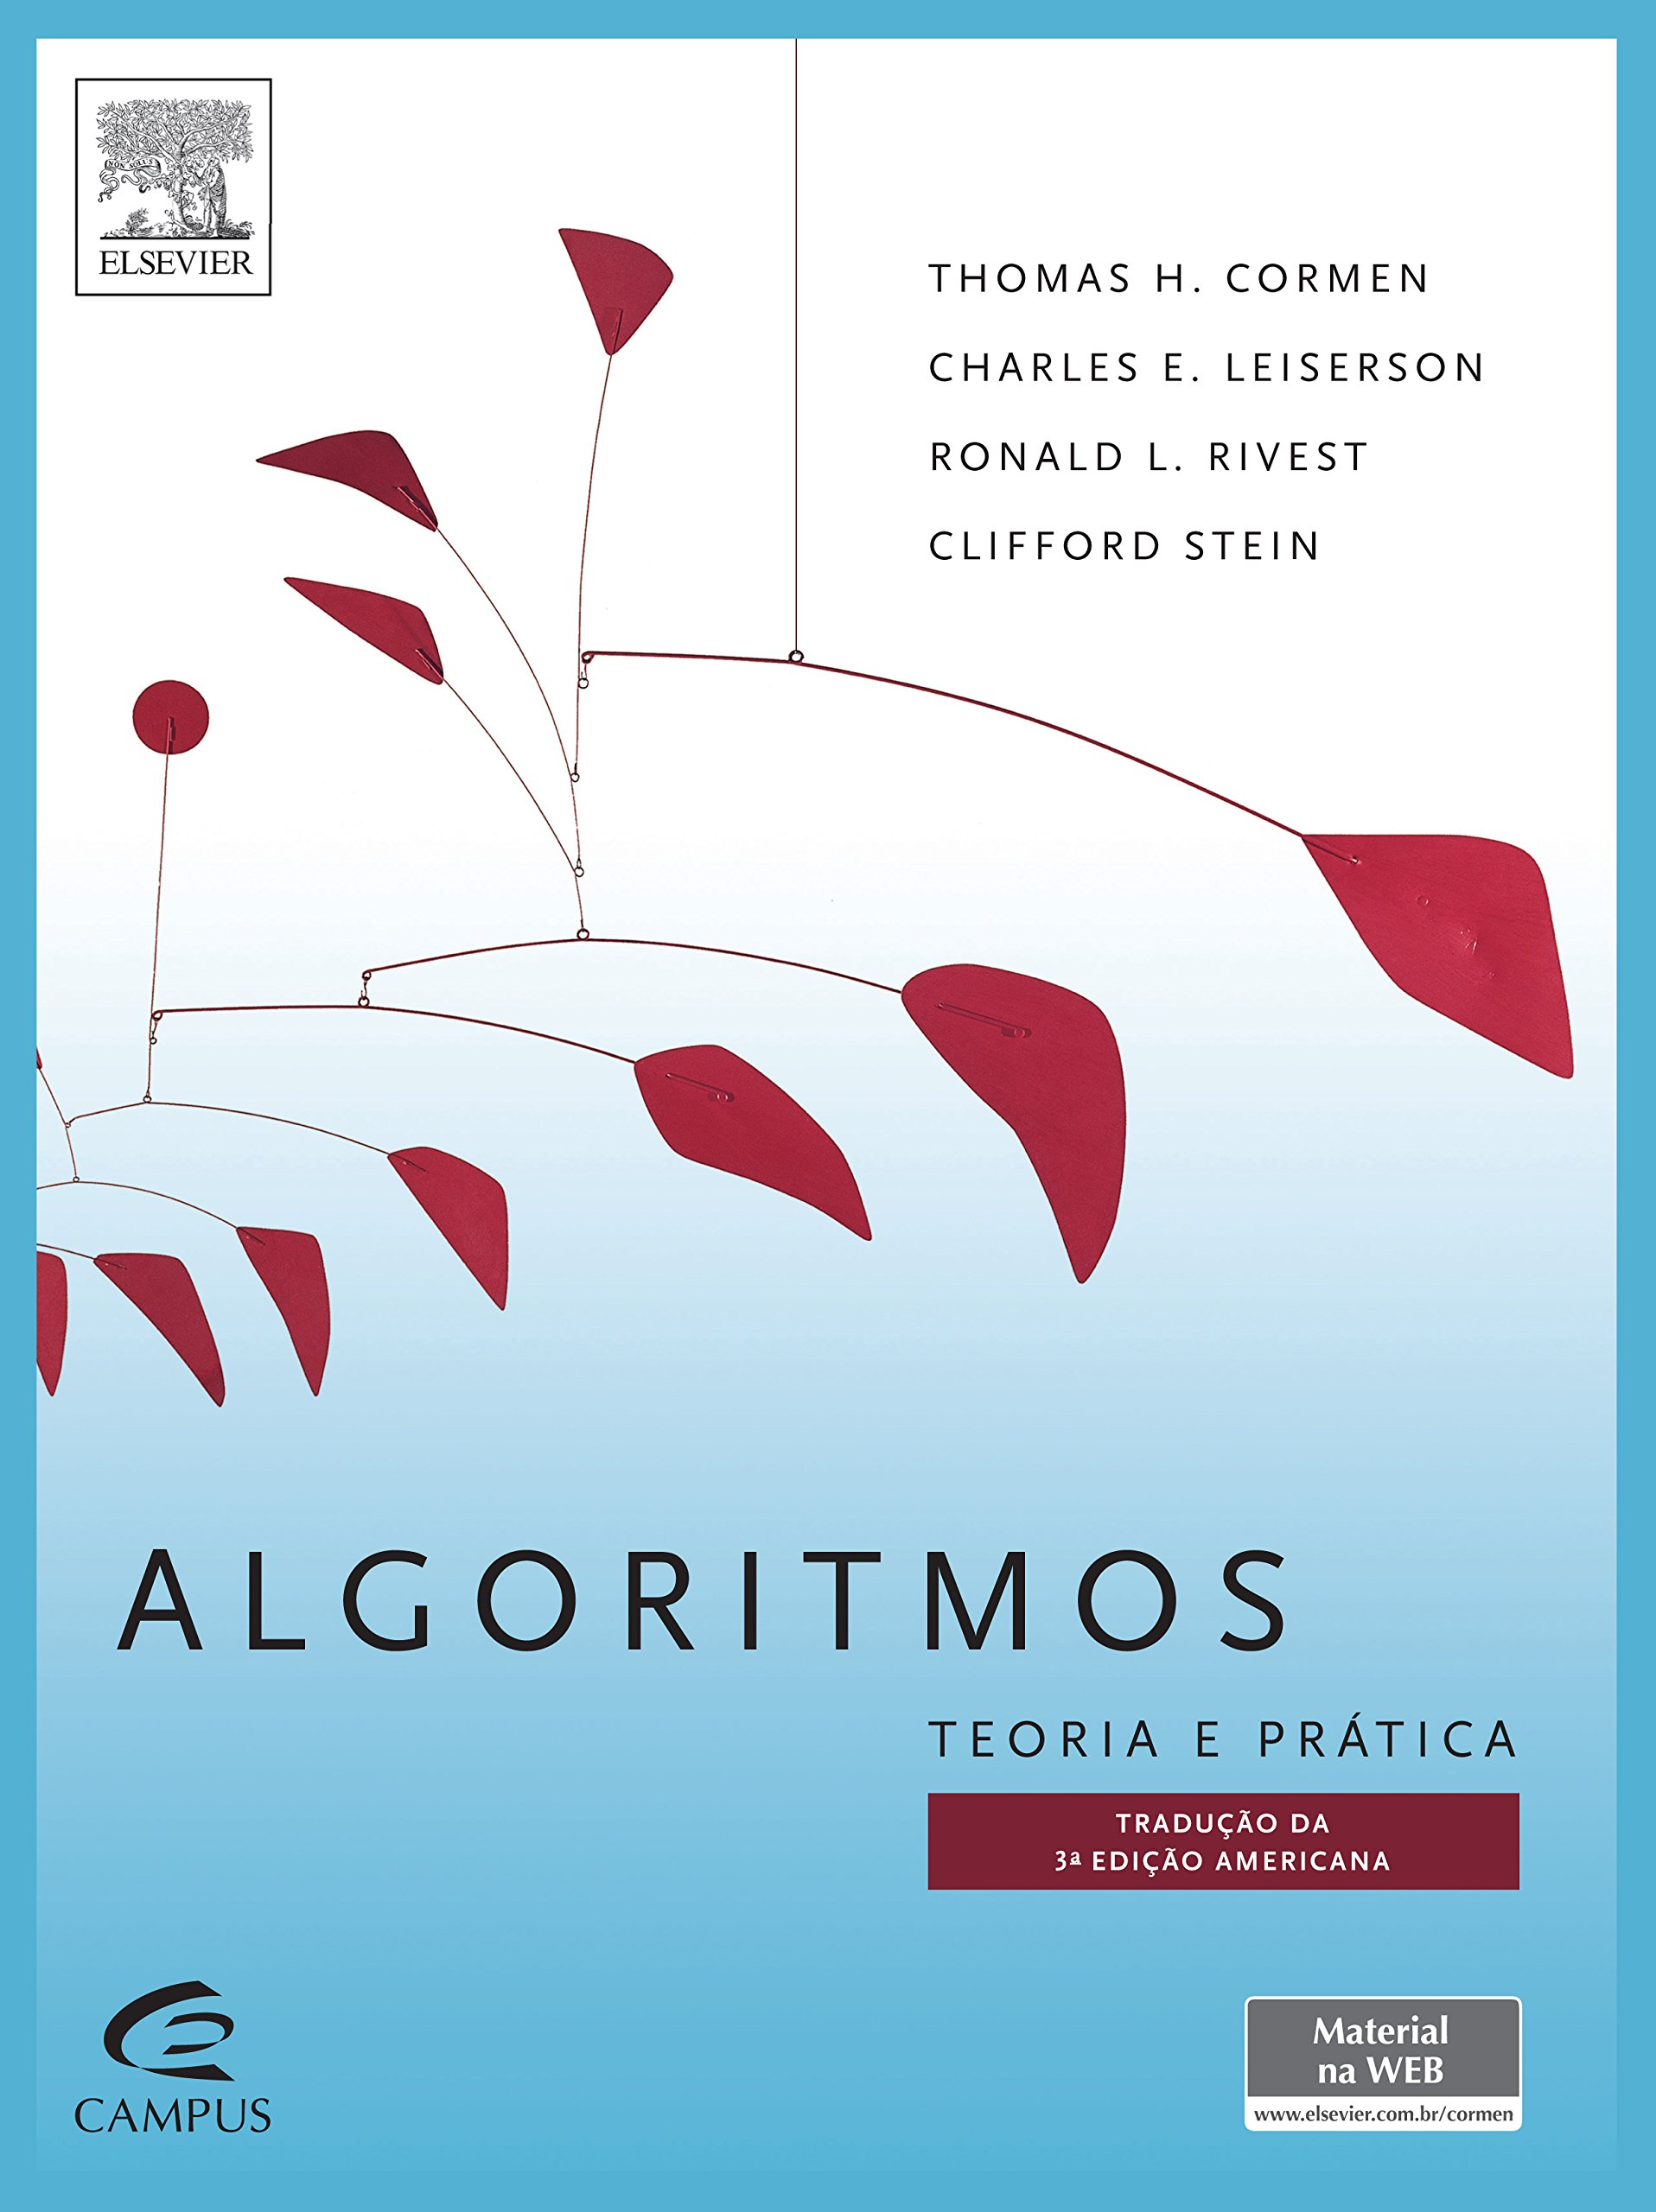
\includegraphics[scale=0.05]{cormen.jpg}
    \end{minipage}
    \begin{minipage}{0.5\textwidth}
        \begin{small}
            \begin{tabularx}{0.98\textwidth}{lX}
                \textbf{Autor:} & Thomas H. Cormen \\
                \textbf{1ª Edição:} & 1989  \\
                \textbf{Volumes:} & 1 \\
                \textbf{Páginas:} & 944 \\
                \textbf{Nível:} & Intermediário \\
            \end{tabularx}
        \end{small}
    \end{minipage}

    \vspace{0.2in} 

    Livro texto dos cursos de algoritmos da melhores universidades do mundo, e é uma obra
    de referência e consulta para os profissionais da área. 

\end{frame}

\begin{frame}[fragile]{The C Programming Language}

    \begin{minipage}{0.4\textwidth}
        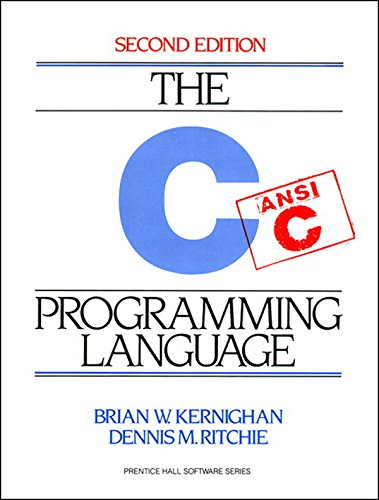
\includegraphics[scale=0.25]{kr.jpg}
    \end{minipage}
    \begin{minipage}{0.5\textwidth}
        \begin{small}
            \begin{tabularx}{0.95\textwidth}{lX}
                \textbf{Autores:} & Brian W. Kernighan \\
                & Denis M. Ritchie \\
                \textbf{1ª Edição:} & 1978 \\
                \textbf{Volumes:} & 1 \\
                \textbf{Páginas:} & 279 \\
                \textbf{Nível:} & Introdutório \\
            \end{tabularx}
        \end{small}
    \end{minipage}

    \vspace{0.2in} 

    Livro sobre a linguagem C escrito pelos autores da linguagem. Leitura fácil e
    didática. A obra se tornou a referência do C antes da padronização.

\end{frame}

\begin{frame}[fragile]{The C++ Programming Language}

    \begin{minipage}{0.4\textwidth}
        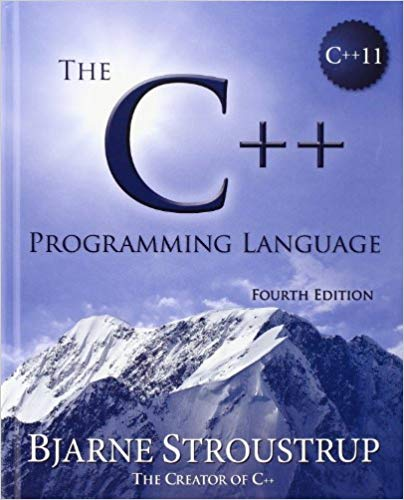
\includegraphics[scale=0.25]{bjarne.jpg}
    \end{minipage}
    \begin{minipage}{0.5\textwidth}
        \begin{small}
            \begin{tabularx}{0.95\textwidth}{lX}
                \textbf{Autor:} & Bjarne Stroustroup \\
                \textbf{1ª Edição:} & 1985 \\
                \textbf{Volumes:} & 1 \\
                \textbf{Páginas:} & 1346 \\
                \textbf{Nível:} & Intermediário \\
            \end{tabularx}
        \end{small}
    \end{minipage}

    \vspace{0.2in} 

    Livro sobre C++ escrito pelo autor da linguagem. A escrita é técnica e detalhada,
    e exige bastante do leitor.

\end{frame}

\begin{frame}[fragile]{Effective C++}

    \begin{minipage}{0.4\textwidth}
        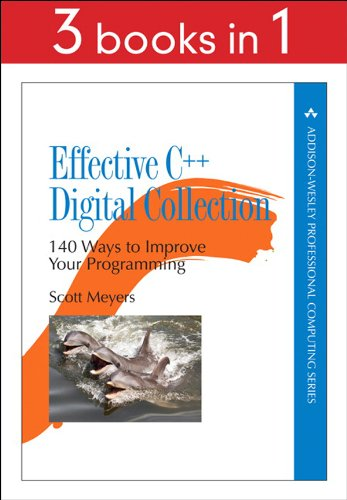
\includegraphics[scale=0.25]{scott.jpg}
    \end{minipage}
    \begin{minipage}{0.5\textwidth}
        \begin{small}
            \begin{tabularx}{0.95\textwidth}{lX}
                \textbf{Autor:} & Scott Meyers \\
                \textbf{1ª Edição:} & 1992 \\
                \textbf{Volumes:} & 4 \\
                \textbf{Páginas:} & 2796 \\
                \textbf{Nível:} & Intermediário \\
            \end{tabularx}
        \end{small}
    \end{minipage}

    \vspace{0.2in} 

    Quatro livros sobre técnicas efetivas para C++: \textit{Effective C++, More Effective C++,
    Effective STL, Effective Modern C++}. O autor é didático, mas a leitura exige um bom
    conhecimento prévio de C++ para melhor entendimento da discussão.

\end{frame}

\begin{frame}[fragile]{Clean Code}

    \begin{minipage}{0.4\textwidth}
        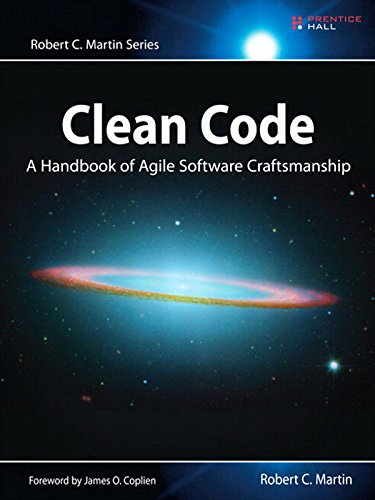
\includegraphics[scale=0.25]{martin.jpg}
    \end{minipage}
    \begin{minipage}{0.5\textwidth}
        \begin{small}
            \begin{tabularx}{0.95\textwidth}{lX}
                \textbf{Autor:} & Robert C. Martin \\
                \textbf{1ª Edição:} & 2008 \\
                \textbf{Volumes:} & 3 \\
                \textbf{Páginas:} & 1105 \\
                \textbf{Nível:} & Introdutório \\
            \end{tabularx}
        \end{small}
    \end{minipage}

    \vspace{0.2in} 

    Série de livros sobre boas práticas de Engenharia de Software (\textit{Clean Code,
    Clean Coder, Clean Architecture}). Leitura obrigatória para estudantes da área.

\end{frame}

\begin{frame}[fragile]{The Pragmatic Programmer: From Journeyman to Master}

    \begin{minipage}{0.4\textwidth}
        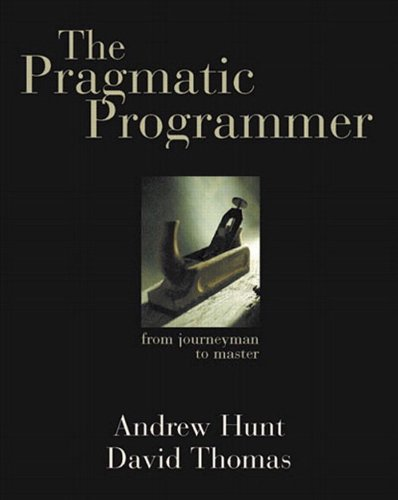
\includegraphics[scale=0.25]{hunt.jpg}
    \end{minipage}
    \begin{minipage}{0.5\textwidth}
        \begin{small}
            \begin{tabularx}{0.95\textwidth}{lX}
                \textbf{Autores:} & Andrew Hunt \\
                & David Thomas \\
                \textbf{1ª Edição:} & 1999 \\
                \textbf{Volumes:} & 1 \\
                \textbf{Páginas:} & 352 \\
                \textbf{Nível:} & Introdutório \\
            \end{tabularx}
        \end{small}
    \end{minipage}

    \vspace{0.2in} 

    Livro bastante influente na área de Engenharia de Software, sendo adotado como livro-texto
    de disciplinas da área. Reune uma série de dicas e métodos para o desenvolvimento de
    software.

\end{frame}

\begin{frame}[fragile]{Refactoring: Improving the Design of Existing Code}

    \begin{minipage}{0.4\textwidth}
        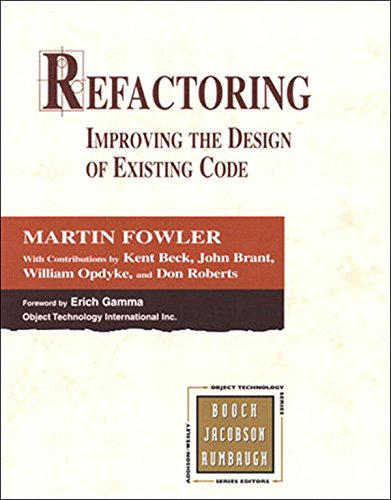
\includegraphics[scale=0.25]{fowler.jpg}
    \end{minipage}
    \begin{minipage}{0.5\textwidth}
        \begin{small}
            \begin{tabularx}{0.95\textwidth}{lX}
                \textbf{Autores:} & Martin Fowler \\
                & Kent Beck \\
                & John Brant \\
                & William Opdyke \\
                \textbf{1ª Edição:} & 1999 \\
                \textbf{Volumes:} & 1 \\
                \textbf{Páginas:} & 461 \\
                \textbf{Nível:} & Introdutório \\
            \end{tabularx}
        \end{small}
    \end{minipage}

    \vspace{0.2in} 

    Livro que introduz a técnica de refatorção de código. Obrigatório para estudantes de
    Engenharia de Software.
\end{frame}

\begin{frame}[fragile]{Extreme Programming Explained: Embrace Changes}

    \begin{minipage}{0.4\textwidth}
        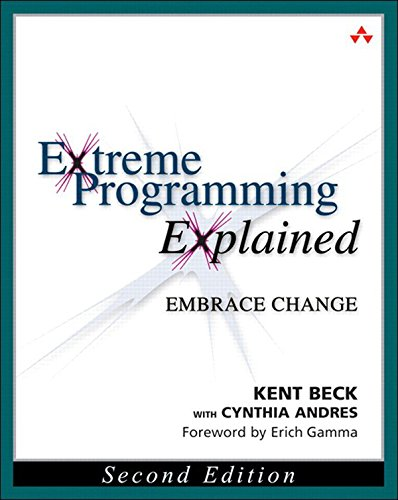
\includegraphics[scale=0.25]{xp.jpg}
    \end{minipage}
    \begin{minipage}{0.5\textwidth}
        \begin{small}
            \begin{tabularx}{0.95\textwidth}{lX}
                \textbf{Autor:} & Kent Beck \\
                & Cynthia Andres \\
                \textbf{1ª Edição:} & 1999 \\
                \textbf{Volumes:} & 1 \\
                \textbf{Páginas:} & 218 \\
                \textbf{Nível:} & Introdutório \\
            \end{tabularx}
        \end{small}
    \end{minipage}

    \vspace{0.2in} 

    Livro que apresenta a \textit{eXtreme Programming} (XP). Obrigatório para estudantes de
    Engenharia de Software.

\end{frame}

\begin{frame}[fragile]{Design Patterns: Elements of Reusable Object-Oriented Software}

    \begin{minipage}{0.4\textwidth}
        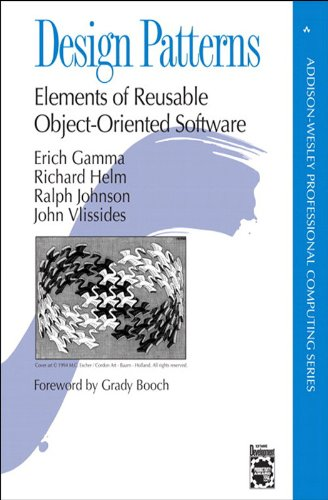
\includegraphics[scale=0.25]{gang.jpg}
    \end{minipage}
    \begin{minipage}{0.5\textwidth}
        \begin{small}
            \begin{tabularx}{0.95\textwidth}{lX}
                \textbf{Autores:} & Erich Gamma \\
                & Richard Helm \\
                & Ralph Jonhson \\
                & John Vlissides \\
                \textbf{1ª Edição:} & 1994 \\
                \textbf{Volumes:} & 1 \\
                \textbf{Páginas:} & 416 \\
                \textbf{Nível:} & Intermediário \\
            \end{tabularx}
        \end{small}
    \end{minipage}

    \vspace{0.2in} 

    Livro escrito pelos autores conhecidos como \textit{Gang of Four}, introduz de forma
    sistemática os padrões de projeto da programação orientada à objetos. Leitura
    obrigatório para os estudadntes de Engenharia de Software.
\end{frame}

\begin{frame}[fragile]{Code Complete}

    \begin{minipage}{0.4\textwidth}
        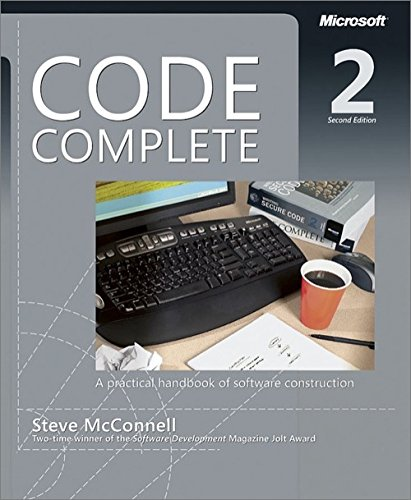
\includegraphics[scale=0.25]{steve.jpg}
    \end{minipage}
    \begin{minipage}{0.5\textwidth}
        \begin{small}
            \begin{tabularx}{0.95\textwidth}{lX}
                \textbf{Autor:} & Steve McConnell \\
                \textbf{1ª Edição:} & 1993 \\
                \textbf{Volumes:} & 1 \\
                \textbf{Páginas:} & 914 \\
                \textbf{Nível:} & Introdutório \\
            \end{tabularx}
        \end{small}
    \end{minipage}

    \vspace{0.2in} 

    Escrito por um experiente programador da Microsoft, é considerado um dos melhores guias
    sobre boas prática de programação.

\end{frame}

\begin{frame}[fragile]{Structure and Interpretation of Computer Programs}

    \begin{minipage}{0.4\textwidth}
        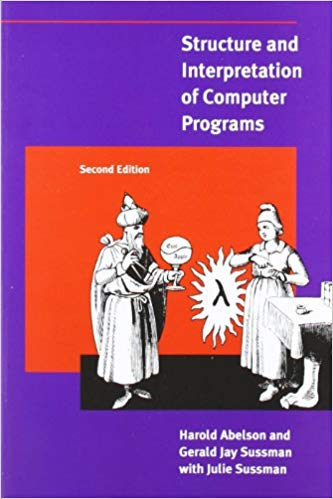
\includegraphics[scale=0.25]{harold.jpg}
    \end{minipage}
    \begin{minipage}{0.5\textwidth}
        \begin{small}
            \begin{tabularx}{0.95\textwidth}{lX}
                \textbf{Autores:} & Harold Abelson \\
                & Gerald Jay Sussman \\
                & Julie Sussman \\
                \textbf{1ª Edição:} & 1979 \\
                \textbf{Volumes:} & 1 \\
                \textbf{Páginas:} & 657 \\
                \textbf{Nível:} & Intermediário \\
            \end{tabularx}
        \end{small}
    \end{minipage}

    \vspace{0.2in} 

    Considerado um dos livros mais influentes da Ciência da Computação, impactou o
    currículo de cursos de grandes universidades desde seu lançamento.

\end{frame}

\begin{frame}[fragile]{The Mythical Man-Month: Essays on Software Engineering}

    \begin{minipage}{0.4\textwidth}
        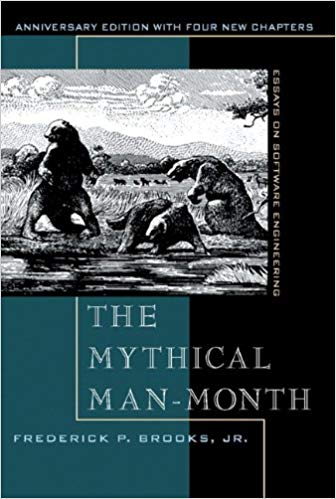
\includegraphics[scale=0.25]{brooks.jpg}
    \end{minipage}
    \begin{minipage}{0.5\textwidth}
        \begin{small}
            \begin{tabularx}{0.95\textwidth}{lX}
                \textbf{Autor:} & Frederick P. Brooks \\
                \textbf{1ª Edição:} & 1975 \\
                \textbf{Volumes:} & 1 \\
                \textbf{Páginas:} & 336 \\
                \textbf{Nível:} & Introdutório \\
            \end{tabularx}
        \end{small}
    \end{minipage}

    \vspace{0.2in} 

    Considerado um clássico da Engenharia de Software, traz ensaios sobre desenvolvimento de
    software e gerência de projetos, e trata do problema da escalabilidade do trabalho
    colaborativo e da natureza de indivíduos e grupos.
\end{frame}

\begin{frame}[fragile]{Compilers: Principles, Techniques, and Tools}

    \begin{minipage}{0.4\textwidth}
        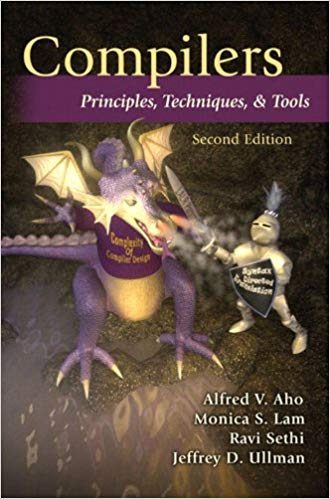
\includegraphics[scale=0.25]{aho.jpg}
    \end{minipage}
    \begin{minipage}{0.5\textwidth}
        \begin{small}
            \begin{tabularx}{0.95\textwidth}{lX}
                \textbf{Autores:} & Alfred V. Aho \\
                & Monica S. Lam \\
                & Ravi Sethi \\
                \textbf{1ª Edição:} & 1986 \\
                \textbf{Volumes:} & 1 \\
                \textbf{Páginas:} & 1009 \\
                \textbf{Nível:} & Avançado \\
            \end{tabularx}
        \end{small}
    \end{minipage}

    \vspace{0.2in} 

    Conhecido como \textit{Dragon Book} (por conta da ilustração da capa), é o livro referência
    sobre compiladores nas melhores universidades do mundo.

\end{frame}

\begin{frame}[fragile]{Redes de Computadores}

    \begin{minipage}{0.35\textwidth}
        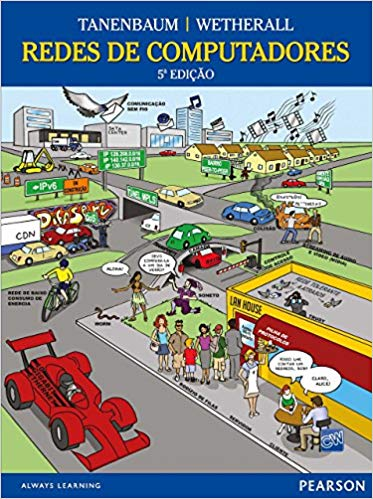
\includegraphics[scale=0.25]{redes.jpg}
    \end{minipage}
    \begin{minipage}{0.55\textwidth}
        \begin{small}
            \begin{tabularx}{0.95\textwidth}{lX}
                \textbf{Autores:} & Andrew S. Tanenbaum \\
                & David Wetherall \\
                \textbf{1ª Edição:} & 1981 \\
                \textbf{Volumes:} & 1 \\
                \textbf{Páginas:} & 600 \\
                \textbf{Nível:} & Intermediário \\
            \end{tabularx}
        \end{small}
    \end{minipage}

    \vspace{0.2in} 

    Livro referência sobre redes de computadores. 

\end{frame}

\begin{frame}[fragile]{Sistemas Operacionais Modernos}

    \begin{minipage}{0.35\textwidth}
        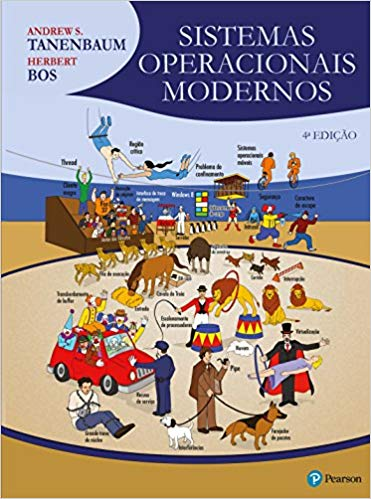
\includegraphics[scale=0.25]{so.jpg}
    \end{minipage}
    \begin{minipage}{0.55\textwidth}
        \begin{small}
            \begin{tabularx}{0.95\textwidth}{lX}
                \textbf{Autor:} & Andrew S. Tanenbaum \\
                \textbf{1ª Edição:} & 1992 \\
                \textbf{Volumes:} & 1 \\
                \textbf{Páginas:} & 864 \\
                \textbf{Nível:} & Avançado \\
            \end{tabularx}
        \end{small}
    \end{minipage}

    \vspace{0.2in} 

    Livro referência sobre sistemas operacionais. Escrito pelo pai do sistema MINIX.

\end{frame}

\begin{frame}[fragile]{Engenharia de Software: Uma Abordagem Profissional}

    \begin{minipage}{0.4\textwidth}
        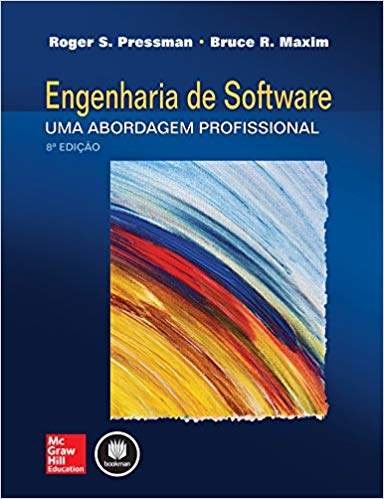
\includegraphics[scale=0.25]{pressman.jpg}
    \end{minipage}
    \begin{minipage}{0.5\textwidth}
        \begin{small}
            \begin{tabularx}{0.95\textwidth}{lX}
                \textbf{Autores:} & Roger S. Pressman \\
                & Bruce R. Maxim \\
                \textbf{1ª Edição:} & 1982 \\
                \textbf{Volumes:} & 1 \\
                \textbf{Páginas:} & 968 \\
                \textbf{Nível:} & Introdutório \\
            \end{tabularx}
        \end{small}
    \end{minipage}

    \vspace{0.2in} 

    Há mais de três décadas o livro introdutório sobre Engenharia de Software. Faz parte da
    ementa de várias disciplinas dos cursos da área.
\end{frame}

\begin{frame}[fragile]{Engenharia de software}

    \begin{minipage}{0.4\textwidth}
        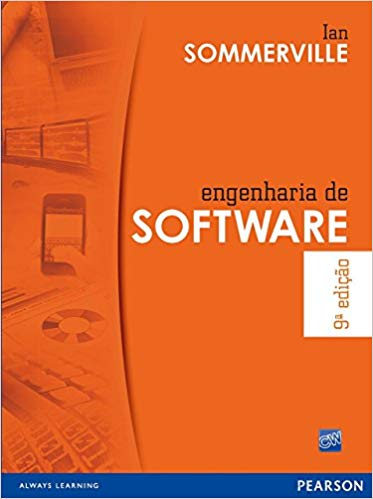
\includegraphics[scale=0.25]{sommerville.jpg}
    \end{minipage}
    \begin{minipage}{0.5\textwidth}
        \begin{small}
            \begin{tabularx}{0.95\textwidth}{lX}
                \textbf{Autor:} & Ian Sommerville \\
                \textbf{1ª Edição:} & 1982 \\
                \textbf{Volumes:} & 1 \\
                \textbf{Páginas:} & 529 \\
                \textbf{Nível:} & Introdutório \\
            \end{tabularx}
        \end{small}
    \end{minipage}

    \vspace{0.2in} 

    Outra grande referência da área de Engenharia de Software, também presente na ementa de
    várias disciplinas dos cursos de graduação.

\end{frame}

\begin{frame}[fragile]{UML Essencial. Um Breve Guia Para a Linguagem-Padrão de Modelagem Para Objetos}

    \begin{minipage}{0.4\textwidth}
        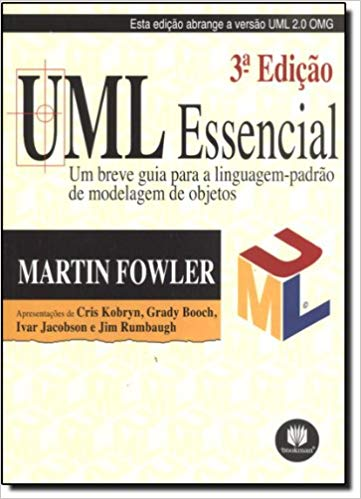
\includegraphics[scale=0.25]{uml.jpg}
    \end{minipage}
    \begin{minipage}{0.5\textwidth}
        \begin{small}
            \begin{tabularx}{0.95\textwidth}{lX}
                \textbf{Autor:} & Martin Fowler \\
                \textbf{1ª Edição:} & 1997 \\
                \textbf{Volumes:} & 1 \\
                \textbf{Páginas:} & 162 \\
                \textbf{Nível:} & Introdutório \\
            \end{tabularx}
        \end{small}
    \end{minipage}

    \vspace{0.2in} 

    Primeiro livro publicado sobre UML, traz a explicação dos principais diagramas. Leitura
    fácil e didática.

\end{frame}

\begin{frame}[fragile]{The Algorithm Design Manual}

    \begin{minipage}{0.4\textwidth}
        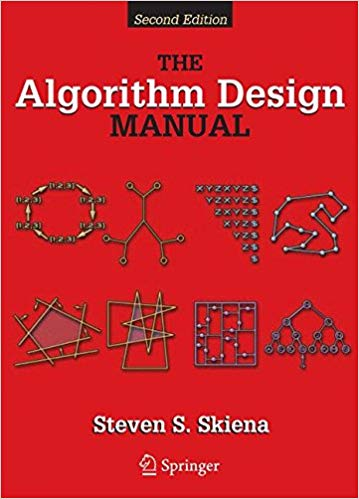
\includegraphics[scale=0.25]{skiena.jpg}
    \end{minipage}
    \begin{minipage}{0.5\textwidth}
        \begin{small}
            \begin{tabularx}{0.95\textwidth}{lX}
                \textbf{Autor:} & Steven S. Skiena \\
                \textbf{1ª Edição:} & 1997 \\
                \textbf{Volumes:} & 1 \\
                \textbf{Páginas:} & 730 \\
                \textbf{Nível:} & Intermediário \\
            \end{tabularx}
        \end{small}
    \end{minipage}

    \vspace{0.2in} 

    Excelente livro sobre projeto e análise de algoritmos.

\end{frame}

\begin{frame}[fragile]{Scrum. A Arte de Fazer o Dobro do Trabalho na Metade do Tempo}

    \begin{minipage}{0.4\textwidth}
        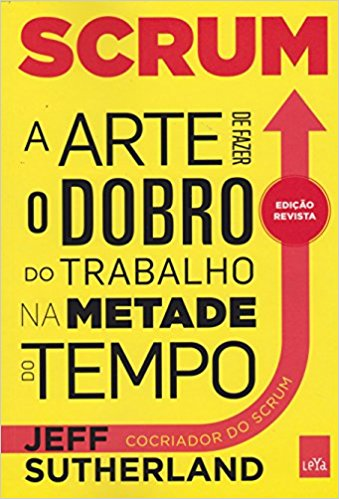
\includegraphics[scale=0.25]{scrum.jpg}
    \end{minipage}
    \begin{minipage}{0.5\textwidth}
        \begin{small}
            \begin{tabularx}{0.95\textwidth}{lX}
                \textbf{Autor:} & Jeff Sutherland \\
                \textbf{1ª Edição:} & 2014 \\
                \textbf{Volumes:} & 1 \\
                \textbf{Páginas:} & 240 \\
                \textbf{Nível:} & Introdutório \\
            \end{tabularx}
        \end{small}
    \end{minipage}

    \vspace{0.2in} 

    Livro sobre o SCRUM, por um de seus idealizadores.

\end{frame}

